\begin{figure}[t]
	\centering
	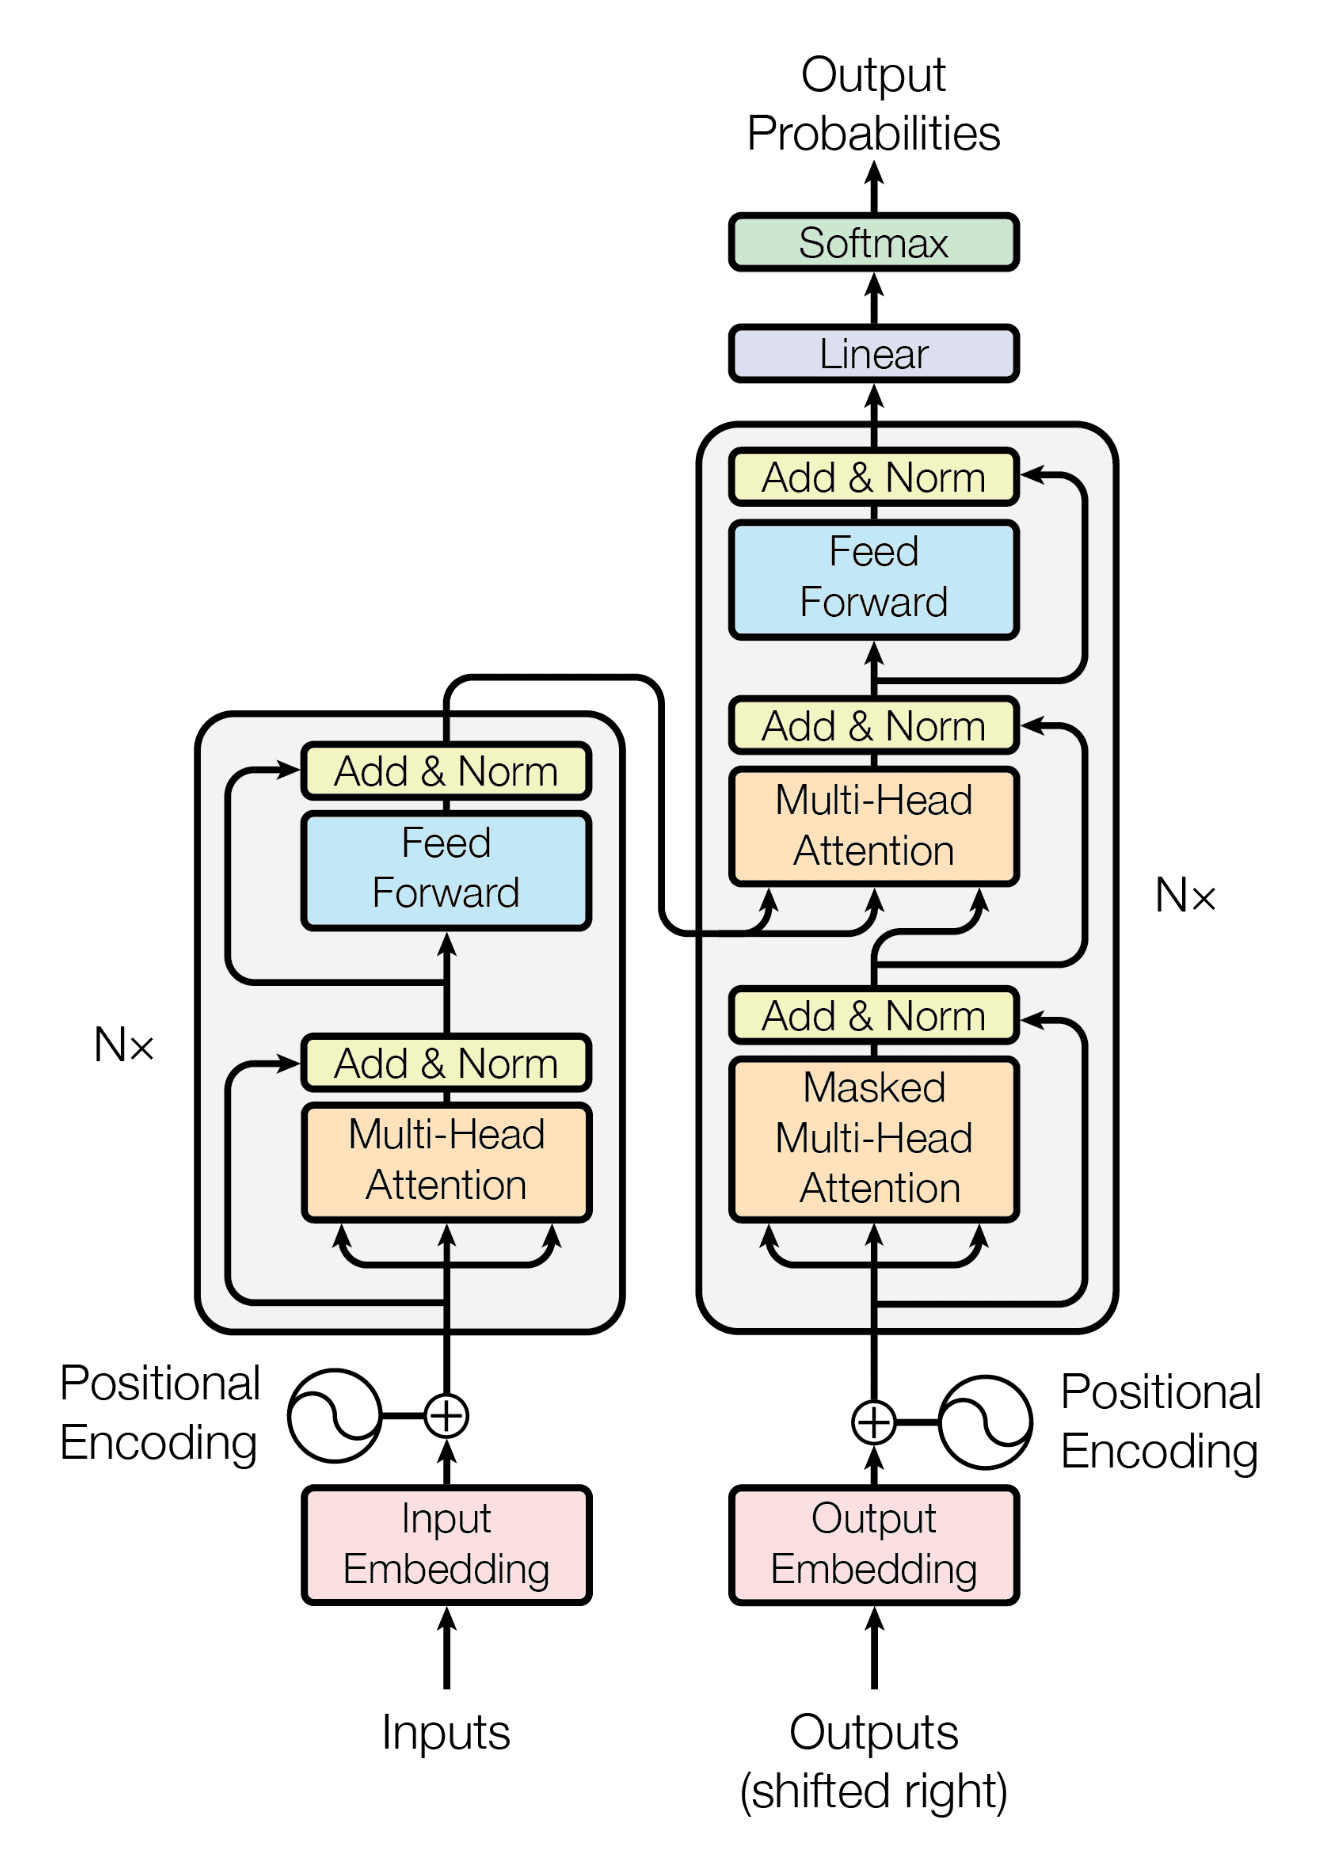
\includegraphics[scale=0.2]{./images/transformer/transformer.png}
	\caption{An illustration of Transformer architecture.}
\end{figure}

\paragraph{TLDR}
\begin{itemize}
	\item \textit{Attention is a communication mechanism}, which can be seen as nodes in a directed graph looking at each other and aggregating information with a weighted sum from all nodes that point to them, with data-dependent weights.
	\item There is no notion of space. Attention simply acts over a set of vectors. This is why we need to positionally encode tokens.
	\item Each example across batch dimension is of course processed completely independently and never ``talk'' to each other
	\item In an ``encoder'' attention block just delete the single line that does masking with `tril`, allowing all tokens to communicate. This block here is called a ``decoder'' attention block because it has triangular masking, and is usually used in autoregressive settings, like language modeling.
	\item ``self-attention'' just means that the keys and values are produced from the same source as queries. In ``cross-attention'', the queries still get produced from $x$, but the keys and values come from some other, external source (\eg an encoder module)
	\item ``Scaled'' attention additional divides `wei` by $1/sqrt(head\_size)$. This makes it so when input Q,K are unit variance, wei will be unit variance too and Softmax will stay diffuse and not saturate too much. Illustration below
\end{itemize}

\section{Attention Mechanism}
\label{sec:nlp_attention}


The attention mechanism assigns \textit{attention scores} (\ie \textit{weights}) to different parts of the input sequence, indicating how much each part contributes to the current output. In essence, the model ``pays attention'' to certain parts of the input more than others while processing each token in the sequence.

Assume the encoder produces 3 hidden states (each a 2-dimensional vector):
\[
h_1 = \begin{bmatrix} 1 \\ 0 \end{bmatrix}, \quad
h_2 = \begin{bmatrix} 0 \\ 1 \end{bmatrix}, \quad
h_3 = \begin{bmatrix} 1 \\ 1 \end{bmatrix}.
\]

Let the decoder’s previous hidden state at time \( t-1 \) be:
\[
s_{t-1} = \begin{bmatrix} 0.5 \\ 0.2 \end{bmatrix}.
\]

Using the \textit{dot product} as our score function, the alignment score for each encoder hidden state is:
\[
e_{tj} = s_{t-1}^\top h_j.
\]

Compute each:
\begin{enumerate}
	\item  For \( h_1 \):
   \[
   e_{t1} = [0.5 \quad 0.2] \cdot \begin{bmatrix} 1 \\ 0 \end{bmatrix} = 0.5.
   \]
\item For \( h_2 \):
   \[
   e_{t2} = [0.5 \quad 0.2] \cdot \begin{bmatrix} 0 \\ 1 \end{bmatrix} = 0.2.
   \]
\item For \( h_3 \):
   \[
   e_{t3} = [0.5 \quad 0.2] \cdot \begin{bmatrix} 1 \\ 1 \end{bmatrix} = 0.7.
   \]
\end{enumerate}

The attention weight for each encoder time step is given by:
\[
\alpha_{tj} = \frac{\exp(e_{tj})}{\sum_{k=1}^{3} \exp(e_{tk})}.
\]

Calculate the exponentials:
\begin{itemize}
	\item \(\exp(0.5) \approx 1.6487\),
	\item \(\exp(0.2) \approx 1.2214\),
	\item \(\exp(0.7) \approx 2.0138\).
\end{itemize}

Sum of exponentials:
\[
S = 1.6487 + 1.2214 + 2.0138 \approx 4.8839.
\]

Now compute each attention weight:
\begin{enumerate}
	\item For \( \alpha_{t1} \):
   \[
   \alpha_{t1} = \frac{1.6487}{4.8839} \approx 0.3374.
   \]
\item For \( \alpha_{t2} \):
   \[
   \alpha_{t2} = \frac{1.2214}{4.8839} \approx 0.2501.
   \]
\item For \( \alpha_{t3} \):
   \[
   \alpha_{t3} = \frac{2.0138}{4.8839} \approx 0.4125.
   \]
\end{enumerate}

These weights sum to 1 (up to rounding):

\[
0.3374 + 0.2501 + 0.4125 \approx 1.0000.
\]

The context vector \( c_t \) is the weighted sum of the encoder hidden states:

\[
c_t = \alpha_{t1} h_1 + \alpha_{t2} h_2 + \alpha_{t3} h_3.
\]

Substitute in the values:

\[
\begin{aligned}
c_t &= 0.3374 \begin{bmatrix} 1 \\ 0 \end{bmatrix} 
+ 0.2501 \begin{bmatrix} 0 \\ 1 \end{bmatrix} 
+ 0.4125 \begin{bmatrix} 1 \\ 1 \end{bmatrix} \\
&= \begin{bmatrix} 0.3374 \\ 0 \end{bmatrix} 
+ \begin{bmatrix} 0 \\ 0.2501 \end{bmatrix} 
+ \begin{bmatrix} 0.4125 \\ 0.4125 \end{bmatrix} \\
&= \begin{bmatrix} 0.3374 + 0.4125 \\ 0 + 0.2501 + 0.4125 \end{bmatrix} \\
&= \begin{bmatrix} 0.7499 \\ 0.6626 \end{bmatrix}.
\end{aligned}
\]

So, the context vector is approximately:

\[
c_t \approx \begin{bmatrix} 0.75 \\ 0.66 \end{bmatrix}.
\]

In a typical decoder, the context vector \( c_t \) is combined with the previous hidden state and possibly the previously generated output to update the current hidden state. For example, an update could be:

\[
s_t = f(s_{t-1}, y_{t-1}, c_t),
\]

or, if you are using a simple formulation with a combined input, it might be:

\[
s_t = \tanh(W [s_{t-1}; c_t]),
\]

where \( [s_{t-1}; c_t] \) denotes the concatenation of \( s_{t-1} \) and \( c_t \), and \( W \) is a learnable weight matrix. The updated state \( s_t \) would then be used to predict the next output token.

Let's use a machine translation task (English to French) as an example. Suppose we are translating the sentence ``I am learning'' into French. 
\begin{itemize}
	\item Input: Sequence of words in English: `[I, am, learning]`
	\item Output: Sequence of words in French: `[Je, suis, en, train, d'apprendre]`
\end{itemize}

Instead of compressing all the input information into a fixed-size context vector (like in traditional encoder-decoder models), the attention mechanism allows the decoder to look at different parts of the input sentence at each step of the decoding process.

\begin{table}[h]
\centering
\begin{tabular}{lccc}
\toprule
& I & am & learning \\
\midrule
Je   & 0.7  & 0.2  & 0.1 \\
suis & 0.1  & 0.8  & 0.1 \\
en   & 0.05 & 0.15 & 0.8 \\
\bottomrule
\end{tabular}
\end{table}

This matrix shows that ``Je'' strongly attends to ``I'', ``suis'' attends mostly to ``am'', and ``en'' attends primarily to ``learning''.

% The encoder's inputs first flow through a self-attention layer – a layer that helps the encoder look at other words in the input sentence as it encodes a specific word. 

\subsection{Self-Attention}
% $$attn(Q,K,V) = softmax\bigg(\frac{Q^TK}{\sqrt{d_k}}\bigg)V$$

\begin{itemize}
	\item \( n \): the number of tokens in the sequence.
	\item \( d_{\text{model}} \): the dimension of the input embeddings.
	\item \( d_k \): the dimension of the query and key vectors.
	\item \( d_v \): the dimension of the value vectors (often \( d_k = d_v \), but they need not be equal).
\end{itemize}

Assume we have an input sequence of \( n \) tokens. For each token \( i \) (with \( 1 \leq i \leq n \)) we start with an embedding vector \( \mathbf{x}_i \in \mathbb{R}^{d_{\text{model}}} \). In self‐attention, we first linearly project these embeddings into three different spaces to obtain the \textit{query}, \textit{key}, and \textit{value} vectors:

\[
\begin{aligned}
\mathbf{q}_i &= \mathbf{x}_i \, W^Q, \\
\mathbf{k}_i &= \mathbf{x}_i \, W^K, \\
\mathbf{v}_i &= \mathbf{x}_i \, W^V,
\end{aligned}
\]
where
\begin{itemize}
	\item \( W^Q, W^K \in \mathbb{R}^{d_{\text{model}} \times d_k} \) are the query and key projection matrices,
	\item \( W^V \in \mathbb{R}^{d_{\text{model}} \times d_v} \) is the value projection matrix,
	\item \( d_k \) (and sometimes \( d_v \)) is a chosen dimensionality for these spaces.
\end{itemize}

For a given token \( i \), we compute its output representation as a weighted sum of the value vectors of all tokens. The weights are determined by the similarity between the query \( \mathbf{q}_i \) and the keys \( \mathbf{k}_j \) of all tokens \( j \) in the sequence.

First, compute the \textit{dot-product scores} between the query for token \( i \) and every key:
\[
s_{ij} = \mathbf{q}_i \cdot \mathbf{k}_j, \quad \text{for } j = 1, 2, \dots, n.
\]

To prevent the dot products from growing too large in magnitude (especially when \( d_k \) is large), we \textit{scale the scores} by \( \sqrt{d_k} \):

\[
\tilde{s}_{ij} = \frac{s_{ij}}{\sqrt{d_k}}.
\]

Next, we apply the softmax function over the scaled scores for token \( i \) to obtain the attention weights \( \alpha_{ij} \):

\[
\alpha_{ij} = \frac{\exp(\tilde{s}_{ij})}{\displaystyle \sum_{l=1}^{n} \exp(\tilde{s}_{il})}.
\]

These weights satisfy \( \sum_{j=1}^{n} \alpha_{ij} = 1 \).

Finally, the output for token \( i \), denoted by \( \mathbf{z}_i \), is the weighted sum of the value vectors:

\[
\mathbf{z}_i = \sum_{j=1}^{n} \alpha_{ij} \, \mathbf{v}_j.
\]

In matrix form for all tokens, if we define matrices \( Q \), \( K \), and \( V \) whose rows are the vectors \( \mathbf{q}_i \), \( \mathbf{k}_i \), and \( \mathbf{v}_i \) respectively, the self-attention operation is:

\[
\text{Attention}(Q, K, V) = \operatorname{softmax}\!\left(\frac{QK^\top}{\sqrt{d_k}}\right) V.
\]

Here, $Q, K, V\in \mathbb{R}^{n\times d_{model}}$, $QK^T$'s time complexity is $O(N^2d)$. This quadratic cost is massive for long input-sequences such as documents to be summarized or character-level inputs.

\begin{figure}[t]
	\centering
	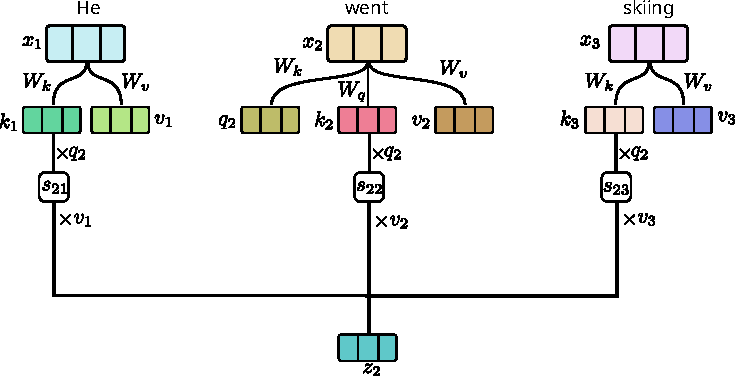
\includegraphics[scale=1.0]{./images/transformer/attention.pdf}
	\caption{An Illustration of the self-attention.}
\end{figure}

\paragraph{Input Embeddings}

   Each token \( i \) is represented by an embedding:
   \[
   \mathbf{x}_i \in \mathbb{R}^{d_{\text{model}}}.
   \]
   
   You can think of all the tokens put together as a matrix:
   \[
   X \in \mathbb{R}^{n \times d_{\text{model}}}.
   \]

\paragraph{Projection Matrices}

   To obtain the queries, keys, and values, we use learned projection matrices:
   \[
   \begin{aligned}
   W^Q &\in \mathbb{R}^{d_{\text{model}} \times d_k}, \\
   W^K &\in \mathbb{R}^{d_{\text{model}} \times d_k}, \\
   W^V &\in \mathbb{R}^{d_{\text{model}} \times d_v}.
   \end{aligned}
   \]

\paragraph{Projected Matrices}
   Multiplying the input \( X \) by these weight matrices gives:
   \[
   \begin{aligned}
   Q &= X\,W^Q \in \mathbb{R}^{n \times d_k}, \\
   K &= X\,W^K \in \mathbb{R}^{n \times d_k}, \\
   V &= X\,W^V \in \mathbb{R}^{n \times d_v}.
   \end{aligned}
   \]
   
   Here, each row of \( Q \) (or \( K \), or \( V \)) corresponds to the query (or key, or value) of one token.

\paragraph{Dot-Product Attention Scores}

   The attention scores between tokens are computed using:
   \[
   QK^\top \in \mathbb{R}^{n \times n}.
   \]
   
   In this product:
   \begin{itemize}
	   \item \( Q \) is \( n \times d_k \)
	   \item \( K^\top \) is \( d_k \times n \)
   \end{itemize}
   
   
   Therefore, the result is an \( n \times n \) matrix where each entry \((i,j)\) represents the (unnormalized) similarity between token \( i \) and token \( j \).

   \paragraph{Scaled Dot-Product and Softmax}

   Before applying the softmax, the scores are scaled by \( \sqrt{d_k} \):
   \[
   \frac{QK^\top}{\sqrt{d_k}} \in \mathbb{R}^{n \times n}.
   \]
   
   Then, applying the softmax function row-wise produces an attention weight matrix \( A \in \mathbb{R}^{n \times n} \):
   \[
   A = \operatorname{softmax}\!\left(\frac{QK^\top}{\sqrt{d_k}}\right).
   \]

   \paragraph{Final Output}
   Finally, the output of the self-attention layer is computed as:
   \[
   \text{Attention}(Q, K, V) = A\,V.
   \]
   
   Since:
   \begin{itemize}
	   \item \( A \) is \( n \times n \),
	   \item \( V \) is \( n \times d_v \),
   \end{itemize}
   
   The final output is:
   \[
   \text{Attention}(Q, K, V) \in \mathbb{R}^{n \times d_v}.
   \]

\subsection{Masked Attention}
In autoregressive tasks (\eg language modeling), it is essential that when predicting a token at position ii, the model does not ``peek'' at any tokens at positions $j>i$. \textit{Masked attention} ensures that each token only attends to tokens at the same or earlier positions. The masked attention is often referred to \textit{cross-attention}. This is just a self-attention in decoder.
$$\textrm{MA}(Q,K,V) = softmax\bigg(\frac{Q^TK+M}{\sqrt{d_k}}\bigg)V,$$
where $M$ 
\begin{align*}
	M_{ij} = \begin{cases}
		0&\text{if } j\leq i\\
		-\infty&\text{if } j>i
	\end{cases}
\end{align*}
Note that $-\infty$ will make $exp$ term to be zero.

\subsection{Multi-Head Attention}
Multi-head attention allows the model to jointly attend to information from different representation subspaces at different positions. \textbf{Rather than computing a single attention function with full-dimensional queries, keys, and values, the mechanism splits them into multiple ``heads'' and computes attention in parallel}. 

Suppose:
\begin{itemize}
	\item The input embeddings (or previous layer outputs) form the matrix \(X \in \mathbb{R}^{n \times d_{\text{model}}}\),
	\item \(d_{\text{model}}\) is the model (or embedding) dimension,
	\item We decide to use \(h\) attention heads.
\end{itemize}

Each head will work with lower-dimensional projections of the input. In particular, we typically set:
\[
d_k' = d_v' = \frac{d_{\text{model}}}{h},
\]
so that each head processes queries, keys, and values of dimensions \(d_k'\) and \(d_v'\), and the total computation remains efficient.

\paragraph{Linear Projections for Each Head}

   For each head \(i \in \{1, \dots, h\}\), we define learned projection matrices:
   \[
   \begin{aligned}
   W_i^Q &\in \mathbb{R}^{d_{\text{model}} \times d_k'}, \\
   W_i^K &\in \mathbb{R}^{d_{\text{model}} \times d_k'}, \\
   W_i^V &\in \mathbb{R}^{d_{\text{model}} \times d_v'}.
   \end{aligned}
   \]
   We then project the input \(X\) to obtain:
   \[
   \begin{aligned}
   Q_i &= X W_i^Q \in \mathbb{R}^{n \times d_k'}, \\
   K_i &= X W_i^K \in \mathbb{R}^{n \times d_k'}, \\
   V_i &= X W_i^V \in \mathbb{R}^{n \times d_v'}.
   \end{aligned}
   \]

\paragraph{Compute Scaled (Masked) Dot-Product Attention for Each Head}

   For each head \(i\), compute:
   \[
   \text{head}_i = \operatorname{Attention}(Q_i, K_i, V_i),
   \]
   where the attention function is defined as:
   \[
   \text{head}_i = \operatorname{softmax}\!\left(\frac{Q_iK_i^\top + M}{\sqrt{d_k'}}\right) V_i.
   \]
   \begin{itemize}
	   \item If masking is not required (\eg in the encoder or in \textit{non-autoregressive} settings), simply set \(M = 0\).
	   \item \textit{For decoder self-attention in autoregressive models}, \(M\) is defined as in the Masked Attention section above.
   \end{itemize}

\paragraph{Concatenate the Heads and Project}

   Once all heads are computed, we concatenate their outputs:
   \[
   \text{Concat}(\text{head}_1, \text{head}_2, \dots, \text{head}_h) \in \mathbb{R}^{n \times (h \cdot d_v')}.
   \]
   Finally, we apply a learned linear projection:
   \[
   W^O \in \mathbb{R}^{(h \cdot d_v') \times d_{\text{model}}},
   \]
   to obtain the final multi-head attention output:
   \[
   \text{MultiHead}(Q, K, V) = \text{Concat}(\text{head}_1, \dots, \text{head}_h) W^O \in \mathbb{R}^{n \times d_{\text{model}}}.
   \]

   % \begin{itemize}
		% \item Input \(X\): \( n \times d_{\text{model}} \)
		% \item Projection matrices \(W_i^Q, W_i^K, W_i^V\): \( d_{\text{model}} \times d_k' \) (or \( d_v' \))
		% \item Projected matrices for each head:
		% \item  \( Q_i, K_i \in \mathbb{R}^{n \times d_k'} \)
		% \item  \( V_i \in \mathbb{R}^{n \times d_v'} \)
		% \item Attention score matrix (per head):
		% \item \( Q_iK_i^\top \in \mathbb{R}^{n \times n} \)
		% \item Output of each head: \( \text{head}_i \in \mathbb{R}^{n \times d_v'} \)
		% \item Concatenated heads: \( n \times (h \cdot d_v') \)
		% \item Final projection \(W^O\): \( (h \cdot d_v') \times d_{\text{model}} \)
		% \item Final multi-head attention output: \( n \times d_{\text{model}} \)
   % \end{itemize}

\section{Various Attention Mechanisms}

\begin{figure}[t]
	\centering
	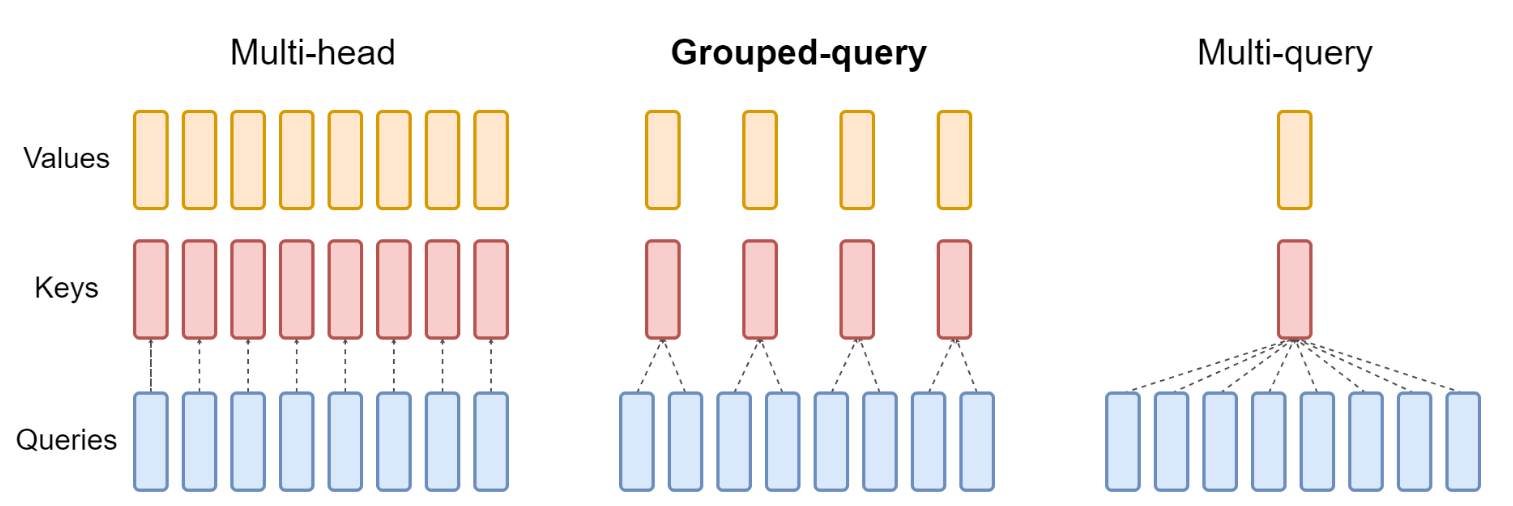
\includegraphics[scale=0.5]{./images/transformer/multi_head_attention.png}
\end{figure}

If we use a single value and a single key over all queries, we can significantly reduce the memory usage for KV caching. This is the basic idea of the multi-query attention (MQA) and the grouped query attention (GQA). However, MQA tends to lower the output quality as the model size increases. GQA achieved a balance between them. 


